\section{Introduction}
%TODO - talk about having to go back to the same location if you want to get good/bad pairs of the ``same'' image.\starnote{I 
assume Cam will
%do this?}
Underwater robotics has been a steadily growing subfield of autonomous field robotics, assisted by the advent of novel platforms,
sensors and propulsion mechanisms. While autonomous underwater vehicles are often equipped with a variety of sensors, visual 
sensing is an
attractive option because of its non-intrusive, passive, and energy efficient nature. The monitoring of coral reefs 
\cite{shkurti2012multi},
deep ocean exploration \cite{whitcomb2000advances}, and mapping of the seabed~\cite{bingham2010robotic} are a number of tasks 
where
visually-guided AUVs and ROVs (Remotely Operated Vehicles) have seen widespread use. Use of these robots ensures humans are not 
exposed to
the hazards of underwater exploration, as they no longer need to venture to the depths (which was how such tasks were carried out 
in the
past). Despite the advantages of using vision, underwater environments pose unique challenges to visual sensing, as phenomena such 
as light
refraction, absorption and scattering from suspended particles can greatly affect the optics of light. As an example, because red
wavelengths are quickly absorbed by water, images tend to have a green or blue hue to them. As one goes deeper, this effect 
worsens, as more
and more red hue is absorbed. This distortion is extremely non-linear in nature, and is affected by a large number of factors, 
such as the
amount of light present (overcast versus sunny, operational depth), amount of particles in the water, time of day, and the camera 
being
used. This may cause difficulty in tasks such as segmentation, tracking, or classification due to their indirect or direct use of 
color.

As color and illumination begin to change with the depth, vision-based algorithms must need to be very generalizable in order to 
work within
the depth ranges a robot may operate in. Because of the high cost and difficulty of acquiring a variety of underwater data to 
train a visual
system on, as well as the high amount of noise introduced, algorithms may (and do) perform poorly in these different
domains. Figure~\ref{fig:samples} shows the high variability in visual scenes that may occur in
underwater environments. A step towards a solution to this issue is to be able to restore the images such that they appear to be 
above
water, \emph{i.e.}, with colors corrected and suspended particles removed from the scene. By performing a many-to-one mapping of 
these
domains from underwater to not underwater (what the image would look like above water), algorithms that have difficulty performing 
across
multiple forms of noise may be able to focus only one clean domain.


\begin{figure}
\centering
\begin{tabular}{p{1.7cm} p{1.7cm} p{1.7cm} p{1.7cm}}
   
   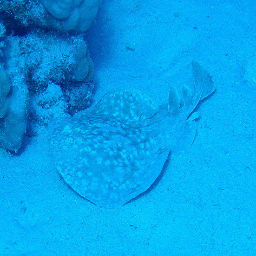
\includegraphics[width=0.8in]{n01496331_7428_f1} &
   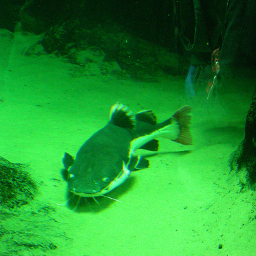
\includegraphics[width=0.8in]{n01496331_16340_f1} &
   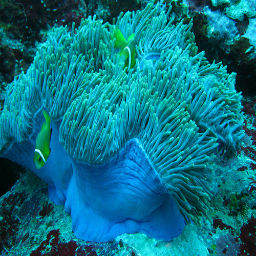
\includegraphics[width=0.8in]{n01914609_5148_f1} &
   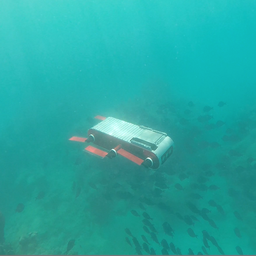
\includegraphics[width=0.8in]{robot_f1} \\
   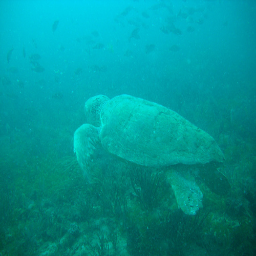
\includegraphics[width=0.8in]{n01664065_30279_f1} &
   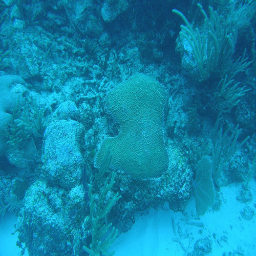
\includegraphics[width=0.8in]{n01917289_5711_f1} &
   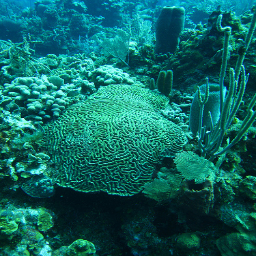
\includegraphics[width=0.8in]{n01917289_4087_f1} &
   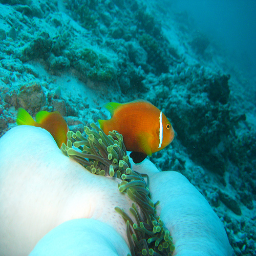
\includegraphics[width=0.8in]{n02607072_10395_f1} \\

\end{tabular}
\label{fig:samples}
\caption{Sample underwater images with natural and man-made artifacts (which in this case is our underwater robot) displaying the 
diversity of distortion that can occur. With the varying camera-to-object distances in the images, the distortion and loss of 
color varies between the different images.}
\end{figure}

Deep neural networks have been shown to be powerful non-linear function approximators, especially in the field of vision 
\cite{krizhevsky2012imagenet}. Often times, these networks require large amounts of data, either labeled or paired with
ground truth. For the problem of automatically colorizing grayscale images \cite{zhang2016colorful}, paired training
data is
readily available due to the fact that any color image can be converted to black and white. However, underwater images distorted 
by either
color or some other phenomenon lack ground truth, which is a major hindrance towards adopting a similar approach for correction. 
This paper proposes a technique based on Generative Adversarial Networks (GANs) to improve the quality of visual underwater scenes 
with the goal of improving the performance of vision-driven behaviors for autonomous underwater robots.
%\starnote{Summarize the approach here. Then talk about datasets as you have done already.}
We use the recently proposed CycleGAN~\cite{zhu2017unpaired} approach, which learns to translate an image from any arbitrary 
domain $X$ to another arbitrary domain $Y$ \textit{without} image pairs, as a way to generate a paired dataset.
By letting $X$ be a set of undistorted underwater images\starnote{need to say where we find the undistorted ones}, and
$Y$ be a set of distorted underwater images, we can generate an image that appears to be underwater while retaining
ground truth.
